% Options for packages loaded elsewhere
\PassOptionsToPackage{unicode}{hyperref}
\PassOptionsToPackage{hyphens}{url}
\PassOptionsToPackage{dvipsnames,svgnames,x11names}{xcolor}
%
\documentclass[
  letterpaper,
  DIV=11,
  numbers=noendperiod,
  oneside]{scrreprt}

\usepackage{amsmath,amssymb}
\usepackage{iftex}
\ifPDFTeX
  \usepackage[T1]{fontenc}
  \usepackage[utf8]{inputenc}
  \usepackage{textcomp} % provide euro and other symbols
\else % if luatex or xetex
  \usepackage{unicode-math}
  \defaultfontfeatures{Scale=MatchLowercase}
  \defaultfontfeatures[\rmfamily]{Ligatures=TeX,Scale=1}
\fi
\usepackage{lmodern}
\ifPDFTeX\else  
    % xetex/luatex font selection
\fi
% Use upquote if available, for straight quotes in verbatim environments
\IfFileExists{upquote.sty}{\usepackage{upquote}}{}
\IfFileExists{microtype.sty}{% use microtype if available
  \usepackage[]{microtype}
  \UseMicrotypeSet[protrusion]{basicmath} % disable protrusion for tt fonts
}{}
\makeatletter
\@ifundefined{KOMAClassName}{% if non-KOMA class
  \IfFileExists{parskip.sty}{%
    \usepackage{parskip}
  }{% else
    \setlength{\parindent}{0pt}
    \setlength{\parskip}{6pt plus 2pt minus 1pt}}
}{% if KOMA class
  \KOMAoptions{parskip=half}}
\makeatother
\usepackage{xcolor}
\usepackage[left=1in,marginparwidth=2.0666666666667in,textwidth=4.1333333333333in,marginparsep=0.3in]{geometry}
\setlength{\emergencystretch}{3em} % prevent overfull lines
\setcounter{secnumdepth}{5}
% Make \paragraph and \subparagraph free-standing
\ifx\paragraph\undefined\else
  \let\oldparagraph\paragraph
  \renewcommand{\paragraph}[1]{\oldparagraph{#1}\mbox{}}
\fi
\ifx\subparagraph\undefined\else
  \let\oldsubparagraph\subparagraph
  \renewcommand{\subparagraph}[1]{\oldsubparagraph{#1}\mbox{}}
\fi

\usepackage{color}
\usepackage{fancyvrb}
\newcommand{\VerbBar}{|}
\newcommand{\VERB}{\Verb[commandchars=\\\{\}]}
\DefineVerbatimEnvironment{Highlighting}{Verbatim}{commandchars=\\\{\}}
% Add ',fontsize=\small' for more characters per line
\usepackage{framed}
\definecolor{shadecolor}{RGB}{241,243,245}
\newenvironment{Shaded}{\begin{snugshade}}{\end{snugshade}}
\newcommand{\AlertTok}[1]{\textcolor[rgb]{0.68,0.00,0.00}{#1}}
\newcommand{\AnnotationTok}[1]{\textcolor[rgb]{0.37,0.37,0.37}{#1}}
\newcommand{\AttributeTok}[1]{\textcolor[rgb]{0.40,0.45,0.13}{#1}}
\newcommand{\BaseNTok}[1]{\textcolor[rgb]{0.68,0.00,0.00}{#1}}
\newcommand{\BuiltInTok}[1]{\textcolor[rgb]{0.00,0.23,0.31}{#1}}
\newcommand{\CharTok}[1]{\textcolor[rgb]{0.13,0.47,0.30}{#1}}
\newcommand{\CommentTok}[1]{\textcolor[rgb]{0.37,0.37,0.37}{#1}}
\newcommand{\CommentVarTok}[1]{\textcolor[rgb]{0.37,0.37,0.37}{\textit{#1}}}
\newcommand{\ConstantTok}[1]{\textcolor[rgb]{0.56,0.35,0.01}{#1}}
\newcommand{\ControlFlowTok}[1]{\textcolor[rgb]{0.00,0.23,0.31}{#1}}
\newcommand{\DataTypeTok}[1]{\textcolor[rgb]{0.68,0.00,0.00}{#1}}
\newcommand{\DecValTok}[1]{\textcolor[rgb]{0.68,0.00,0.00}{#1}}
\newcommand{\DocumentationTok}[1]{\textcolor[rgb]{0.37,0.37,0.37}{\textit{#1}}}
\newcommand{\ErrorTok}[1]{\textcolor[rgb]{0.68,0.00,0.00}{#1}}
\newcommand{\ExtensionTok}[1]{\textcolor[rgb]{0.00,0.23,0.31}{#1}}
\newcommand{\FloatTok}[1]{\textcolor[rgb]{0.68,0.00,0.00}{#1}}
\newcommand{\FunctionTok}[1]{\textcolor[rgb]{0.28,0.35,0.67}{#1}}
\newcommand{\ImportTok}[1]{\textcolor[rgb]{0.00,0.46,0.62}{#1}}
\newcommand{\InformationTok}[1]{\textcolor[rgb]{0.37,0.37,0.37}{#1}}
\newcommand{\KeywordTok}[1]{\textcolor[rgb]{0.00,0.23,0.31}{#1}}
\newcommand{\NormalTok}[1]{\textcolor[rgb]{0.00,0.23,0.31}{#1}}
\newcommand{\OperatorTok}[1]{\textcolor[rgb]{0.37,0.37,0.37}{#1}}
\newcommand{\OtherTok}[1]{\textcolor[rgb]{0.00,0.23,0.31}{#1}}
\newcommand{\PreprocessorTok}[1]{\textcolor[rgb]{0.68,0.00,0.00}{#1}}
\newcommand{\RegionMarkerTok}[1]{\textcolor[rgb]{0.00,0.23,0.31}{#1}}
\newcommand{\SpecialCharTok}[1]{\textcolor[rgb]{0.37,0.37,0.37}{#1}}
\newcommand{\SpecialStringTok}[1]{\textcolor[rgb]{0.13,0.47,0.30}{#1}}
\newcommand{\StringTok}[1]{\textcolor[rgb]{0.13,0.47,0.30}{#1}}
\newcommand{\VariableTok}[1]{\textcolor[rgb]{0.07,0.07,0.07}{#1}}
\newcommand{\VerbatimStringTok}[1]{\textcolor[rgb]{0.13,0.47,0.30}{#1}}
\newcommand{\WarningTok}[1]{\textcolor[rgb]{0.37,0.37,0.37}{\textit{#1}}}

\providecommand{\tightlist}{%
  \setlength{\itemsep}{0pt}\setlength{\parskip}{0pt}}\usepackage{longtable,booktabs,array}
\usepackage{calc} % for calculating minipage widths
% Correct order of tables after \paragraph or \subparagraph
\usepackage{etoolbox}
\makeatletter
\patchcmd\longtable{\par}{\if@noskipsec\mbox{}\fi\par}{}{}
\makeatother
% Allow footnotes in longtable head/foot
\IfFileExists{footnotehyper.sty}{\usepackage{footnotehyper}}{\usepackage{footnote}}
\makesavenoteenv{longtable}
\usepackage{graphicx}
\makeatletter
\def\maxwidth{\ifdim\Gin@nat@width>\linewidth\linewidth\else\Gin@nat@width\fi}
\def\maxheight{\ifdim\Gin@nat@height>\textheight\textheight\else\Gin@nat@height\fi}
\makeatother
% Scale images if necessary, so that they will not overflow the page
% margins by default, and it is still possible to overwrite the defaults
% using explicit options in \includegraphics[width, height, ...]{}
\setkeys{Gin}{width=\maxwidth,height=\maxheight,keepaspectratio}
% Set default figure placement to htbp
\makeatletter
\def\fps@figure{htbp}
\makeatother

\KOMAoption{captions}{tableheading}
\makeatletter
\@ifpackageloaded{tcolorbox}{}{\usepackage[skins,breakable]{tcolorbox}}
\@ifpackageloaded{fontawesome5}{}{\usepackage{fontawesome5}}
\definecolor{quarto-callout-color}{HTML}{909090}
\definecolor{quarto-callout-note-color}{HTML}{0758E5}
\definecolor{quarto-callout-important-color}{HTML}{CC1914}
\definecolor{quarto-callout-warning-color}{HTML}{EB9113}
\definecolor{quarto-callout-tip-color}{HTML}{00A047}
\definecolor{quarto-callout-caution-color}{HTML}{FC5300}
\definecolor{quarto-callout-color-frame}{HTML}{acacac}
\definecolor{quarto-callout-note-color-frame}{HTML}{4582ec}
\definecolor{quarto-callout-important-color-frame}{HTML}{d9534f}
\definecolor{quarto-callout-warning-color-frame}{HTML}{f0ad4e}
\definecolor{quarto-callout-tip-color-frame}{HTML}{02b875}
\definecolor{quarto-callout-caution-color-frame}{HTML}{fd7e14}
\makeatother
\makeatletter
\makeatother
\makeatletter
\@ifpackageloaded{bookmark}{}{\usepackage{bookmark}}
\makeatother
\makeatletter
\@ifpackageloaded{caption}{}{\usepackage{caption}}
\AtBeginDocument{%
\ifdefined\contentsname
  \renewcommand*\contentsname{Table of contents}
\else
  \newcommand\contentsname{Table of contents}
\fi
\ifdefined\listfigurename
  \renewcommand*\listfigurename{List of Figures}
\else
  \newcommand\listfigurename{List of Figures}
\fi
\ifdefined\listtablename
  \renewcommand*\listtablename{List of Tables}
\else
  \newcommand\listtablename{List of Tables}
\fi
\ifdefined\figurename
  \renewcommand*\figurename{Figure}
\else
  \newcommand\figurename{Figure}
\fi
\ifdefined\tablename
  \renewcommand*\tablename{Table}
\else
  \newcommand\tablename{Table}
\fi
}
\@ifpackageloaded{float}{}{\usepackage{float}}
\floatstyle{ruled}
\@ifundefined{c@chapter}{\newfloat{codelisting}{h}{lop}}{\newfloat{codelisting}{h}{lop}[chapter]}
\floatname{codelisting}{Listing}
\newcommand*\listoflistings{\listof{codelisting}{List of Listings}}
\makeatother
\makeatletter
\@ifpackageloaded{caption}{}{\usepackage{caption}}
\@ifpackageloaded{subcaption}{}{\usepackage{subcaption}}
\makeatother
\makeatletter
\@ifpackageloaded{tcolorbox}{}{\usepackage[skins,breakable]{tcolorbox}}
\makeatother
\makeatletter
\@ifundefined{shadecolor}{\definecolor{shadecolor}{rgb}{.97, .97, .97}}
\makeatother
\makeatletter
\makeatother
\makeatletter
\@ifpackageloaded{sidenotes}{}{\usepackage{sidenotes}}
\@ifpackageloaded{marginnote}{}{\usepackage{marginnote}}
\makeatother
\makeatletter
\makeatother
\ifLuaTeX
  \usepackage{selnolig}  % disable illegal ligatures
\fi
\IfFileExists{bookmark.sty}{\usepackage{bookmark}}{\usepackage{hyperref}}
\IfFileExists{xurl.sty}{\usepackage{xurl}}{} % add URL line breaks if available
\urlstyle{same} % disable monospaced font for URLs
\hypersetup{
  pdftitle={Multilevel Multilingual},
  pdfauthor={Andrew Grogan-Kaylor},
  colorlinks=true,
  linkcolor={blue},
  filecolor={Maroon},
  citecolor={Blue},
  urlcolor={Blue},
  pdfcreator={LaTeX via pandoc}}

\title{Multilevel Multilingual}
\author{Andrew Grogan-Kaylor}
\date{2023-11-10}

\begin{document}
\maketitle
\ifdefined\Shaded\renewenvironment{Shaded}{\begin{tcolorbox}[sharp corners, boxrule=0pt, breakable, frame hidden, interior hidden, borderline west={3pt}{0pt}{shadecolor}, enhanced]}{\end{tcolorbox}}\fi

\renewcommand*\contentsname{Table of contents}
{
\hypersetup{linkcolor=}
\setcounter{tocdepth}{2}
\tableofcontents
}
\listoffigures
\listoftables
\bookmarksetup{startatroot}

\hypertarget{multilevel-models-in-stata-r-and-julia}{%
\chapter{Multilevel Models in Stata, R and
Julia}\label{multilevel-models-in-stata-r-and-julia}}

\hypertarget{introduction}{%
\section{Introduction}\label{introduction}}

Below, I describe the use of \href{https://www.stata.com/}{Stata},
\href{https://www.r-project.org/}{R}, and
\href{https://www.julialang.org/}{Julia} to estimate multilevel models.
Because this document is built by
\href{https://quarto.org/}{\texttt{Quarto}}, I describe calling these
programs from within a \texttt{Quarto} environment. However, each piece
of software could be used individually and separately.

\hypertarget{the-data}{%
\section{The Data}\label{the-data}}

\begin{marginfigure}

{\centering 
\includegraphics[width=2.4in,height=\textheight]{bookcover.png}

}

\caption{\label{fig-bookcover}Book Cover For Multilevel Thinking}

\end{marginfigure}

The examples below use the \texttt{simulated\_multilevel\_data.dta} file
from
\href{https://agrogan1.github.io/multilevel-thinking/simulated-multi-country-data.html}{\emph{Multilevel
Thinking}}. Here is a
\href{https://github.com/agrogan1/multilevel-multilingual/raw/main/simulated_multilevel_data.dta}{direct
link} to download the data.

\hypertarget{tbl-multilingual1}{}
\begin{longtable}[]{@{}
  >{\centering\arraybackslash}p{(\columnwidth - 14\tabcolsep) * \real{0.1250}}
  >{\centering\arraybackslash}p{(\columnwidth - 14\tabcolsep) * \real{0.0750}}
  >{\centering\arraybackslash}p{(\columnwidth - 14\tabcolsep) * \real{0.1125}}
  >{\centering\arraybackslash}p{(\columnwidth - 14\tabcolsep) * \real{0.0750}}
  >{\centering\arraybackslash}p{(\columnwidth - 14\tabcolsep) * \real{0.1000}}
  >{\centering\arraybackslash}p{(\columnwidth - 14\tabcolsep) * \real{0.2750}}
  >{\centering\arraybackslash}p{(\columnwidth - 14\tabcolsep) * \real{0.1125}}
  >{\centering\arraybackslash}p{(\columnwidth - 14\tabcolsep) * \real{0.1250}}@{}}
\caption{\label{tbl-multilingual1}Sample of Simulated Multilevel
Data}\tabularnewline
\toprule\noalign{}
\begin{minipage}[b]{\linewidth}\centering
country
\end{minipage} & \begin{minipage}[b]{\linewidth}\centering
HDI
\end{minipage} & \begin{minipage}[b]{\linewidth}\centering
family
\end{minipage} & \begin{minipage}[b]{\linewidth}\centering
id
\end{minipage} & \begin{minipage}[b]{\linewidth}\centering
group
\end{minipage} & \begin{minipage}[b]{\linewidth}\centering
physical\_punishment
\end{minipage} & \begin{minipage}[b]{\linewidth}\centering
warmth
\end{minipage} & \begin{minipage}[b]{\linewidth}\centering
outcome
\end{minipage} \\
\midrule\noalign{}
\endfirsthead
\toprule\noalign{}
\begin{minipage}[b]{\linewidth}\centering
country
\end{minipage} & \begin{minipage}[b]{\linewidth}\centering
HDI
\end{minipage} & \begin{minipage}[b]{\linewidth}\centering
family
\end{minipage} & \begin{minipage}[b]{\linewidth}\centering
id
\end{minipage} & \begin{minipage}[b]{\linewidth}\centering
group
\end{minipage} & \begin{minipage}[b]{\linewidth}\centering
physical\_punishment
\end{minipage} & \begin{minipage}[b]{\linewidth}\centering
warmth
\end{minipage} & \begin{minipage}[b]{\linewidth}\centering
outcome
\end{minipage} \\
\midrule\noalign{}
\endhead
\bottomrule\noalign{}
\endlastfoot
1 & 69 & 1 & 1.1 & 2 & 2 & 3 & 59.18 \\
1 & 69 & 2 & 1.2 & 2 & 4 & 0 & 61.54 \\
1 & 69 & 3 & 1.3 & 1 & 4 & 4 & 51.87 \\
1 & 69 & 4 & 1.4 & 2 & 0 & 6 & 51.71 \\
1 & 69 & 5 & 1.5 & 2 & 3 & 2 & 55.88 \\
1 & 69 & 6 & 1.6 & 1 & 5 & 3 & 60.78 \\
\end{longtable}

\hypertarget{the-equation}{%
\section{The Equation}\label{the-equation}}

\begin{equation}\protect\hypertarget{eq-MLMsubstantive}{}{\text{outcome}_{ij}= \beta_0 + \beta_1 \text{warmth}_{ij} + \beta_2 \text{physical punishment}_{ij} + \\ \beta_3 \text{group}_{ij} + \beta_4 \text{HDI}_{ij} + \\ u_{0j} + u_{1j} \times \text{warmth}_{ij} + e_{ij}}\label{eq-MLMsubstantive}\end{equation}

\hypertarget{setup}{%
\section{Setup}\label{setup}}

\subsection{Stata}

I need to use the library \texttt{Statamarkdown} to call Stata, or I
could run Stata on its own

\begin{Shaded}
\begin{Highlighting}[]
\FunctionTok{library}\NormalTok{(Statamarkdown)}
\end{Highlighting}
\end{Shaded}

\subsection{R}

In R, I use the library \texttt{lme4} to run multilevel models.

\begin{Shaded}
\begin{Highlighting}[]
\FunctionTok{library}\NormalTok{(lme4) }
\end{Highlighting}
\end{Shaded}

\subsection{Julia}

I need to call Julia from R.

\begin{Shaded}
\begin{Highlighting}[]
\FunctionTok{library}\NormalTok{(JuliaCall)}

\FunctionTok{julia\_setup}\NormalTok{(}\AttributeTok{JULIA\_HOME =} \StringTok{"/Applications/Julia{-}1.8.app/Contents/Resources/julia/bin"}\NormalTok{)}
\end{Highlighting}
\end{Shaded}

\hypertarget{get-data-run-models}{%
\section{Get Data \& Run Models}\label{get-data-run-models}}

To explain statistical syntax for each software, I consider the more
general case of a multilevel model with dependent variable \texttt{y},
independent variables \texttt{x} and \texttt{z}, clustering variable
\texttt{group}, and a random slope for \texttt{x}. \emph{i} is the index
for the person, while \emph{j} is the index for the \texttt{group}.

\begin{equation}\protect\hypertarget{eq-MLMsimple}{}{y = \beta_0 + \beta_1 x_{ij} + \beta_2 z_{ij} + u_{0j} + u_{1j} \times x_{ij} + e_{ij}}\label{eq-MLMsimple}\end{equation}

\subsection{Stata}

In Stata \texttt{mixed}, the syntax for a multilevel model of the form
described in Equation~\ref{eq-MLMsimple} is:

\texttt{mixed\ y\ x\ \textbar{}\textbar{}\ group:\ x}

\hypertarget{get-the-data}{%
\subsubsection{Get The Data}\label{get-the-data}}

\begin{tcolorbox}[enhanced jigsaw, arc=.35mm, coltitle=black, bottomtitle=1mm, colbacktitle=quarto-callout-tip-color!10!white, opacityback=0, colback=white, colframe=quarto-callout-tip-color-frame, opacitybacktitle=0.6, breakable, title=\textcolor{quarto-callout-tip-color}{\faLightbulb}\hspace{0.5em}{Tip For Running Stata From Quarto}, leftrule=.75mm, toptitle=1mm, bottomrule=.15mm, rightrule=.15mm, titlerule=0mm, toprule=.15mm, left=2mm]

Because I am running Stata from inside a Quarto document, and running
Stata in multiple chunks, I need to use the \texttt{collectcode=TRUE}
option in the first Stata chunk. i.e.~my Quarto chunk needs to begin
with ```\texttt{\{stata,\ collectcode=TRUE\}}

See Doug Hemken's excellent documentation on \texttt{Statamarkdown}
\href{https://www.ssc.wisc.edu/~hemken/Stataworkshops/Statamarkdown/linking-code-blocks.html\#linking-code-blocks-1}{here}.

\end{tcolorbox}

\begin{Shaded}
\begin{Highlighting}[]

\KeywordTok{use}\NormalTok{ simulated\_multilevel\_data.dta}
\end{Highlighting}
\end{Shaded}

\hypertarget{graph}{%
\subsubsection{Graph}\label{graph}}

\begin{Shaded}
\begin{Highlighting}[]
\KeywordTok{twoway} \KeywordTok{scatter}\NormalTok{ outcome warmth, }\BaseNTok{xtitle}\NormalTok{(}\StringTok{"warmth"}\NormalTok{) }\BaseNTok{ytitle}\NormalTok{(}\StringTok{"outcome"}\NormalTok{) }\BaseNTok{title}\NormalTok{(}\StringTok{"Outcome by Parental Warmth"}\NormalTok{) }

\KeywordTok{quietly} \KeywordTok{graph} \KeywordTok{export} \KeywordTok{scatter}\NormalTok{.png, }\KeywordTok{replace}
\end{Highlighting}
\end{Shaded}

\begin{verbatim}
> arental Warmth") 
\end{verbatim}

\begin{figure}

{\centering 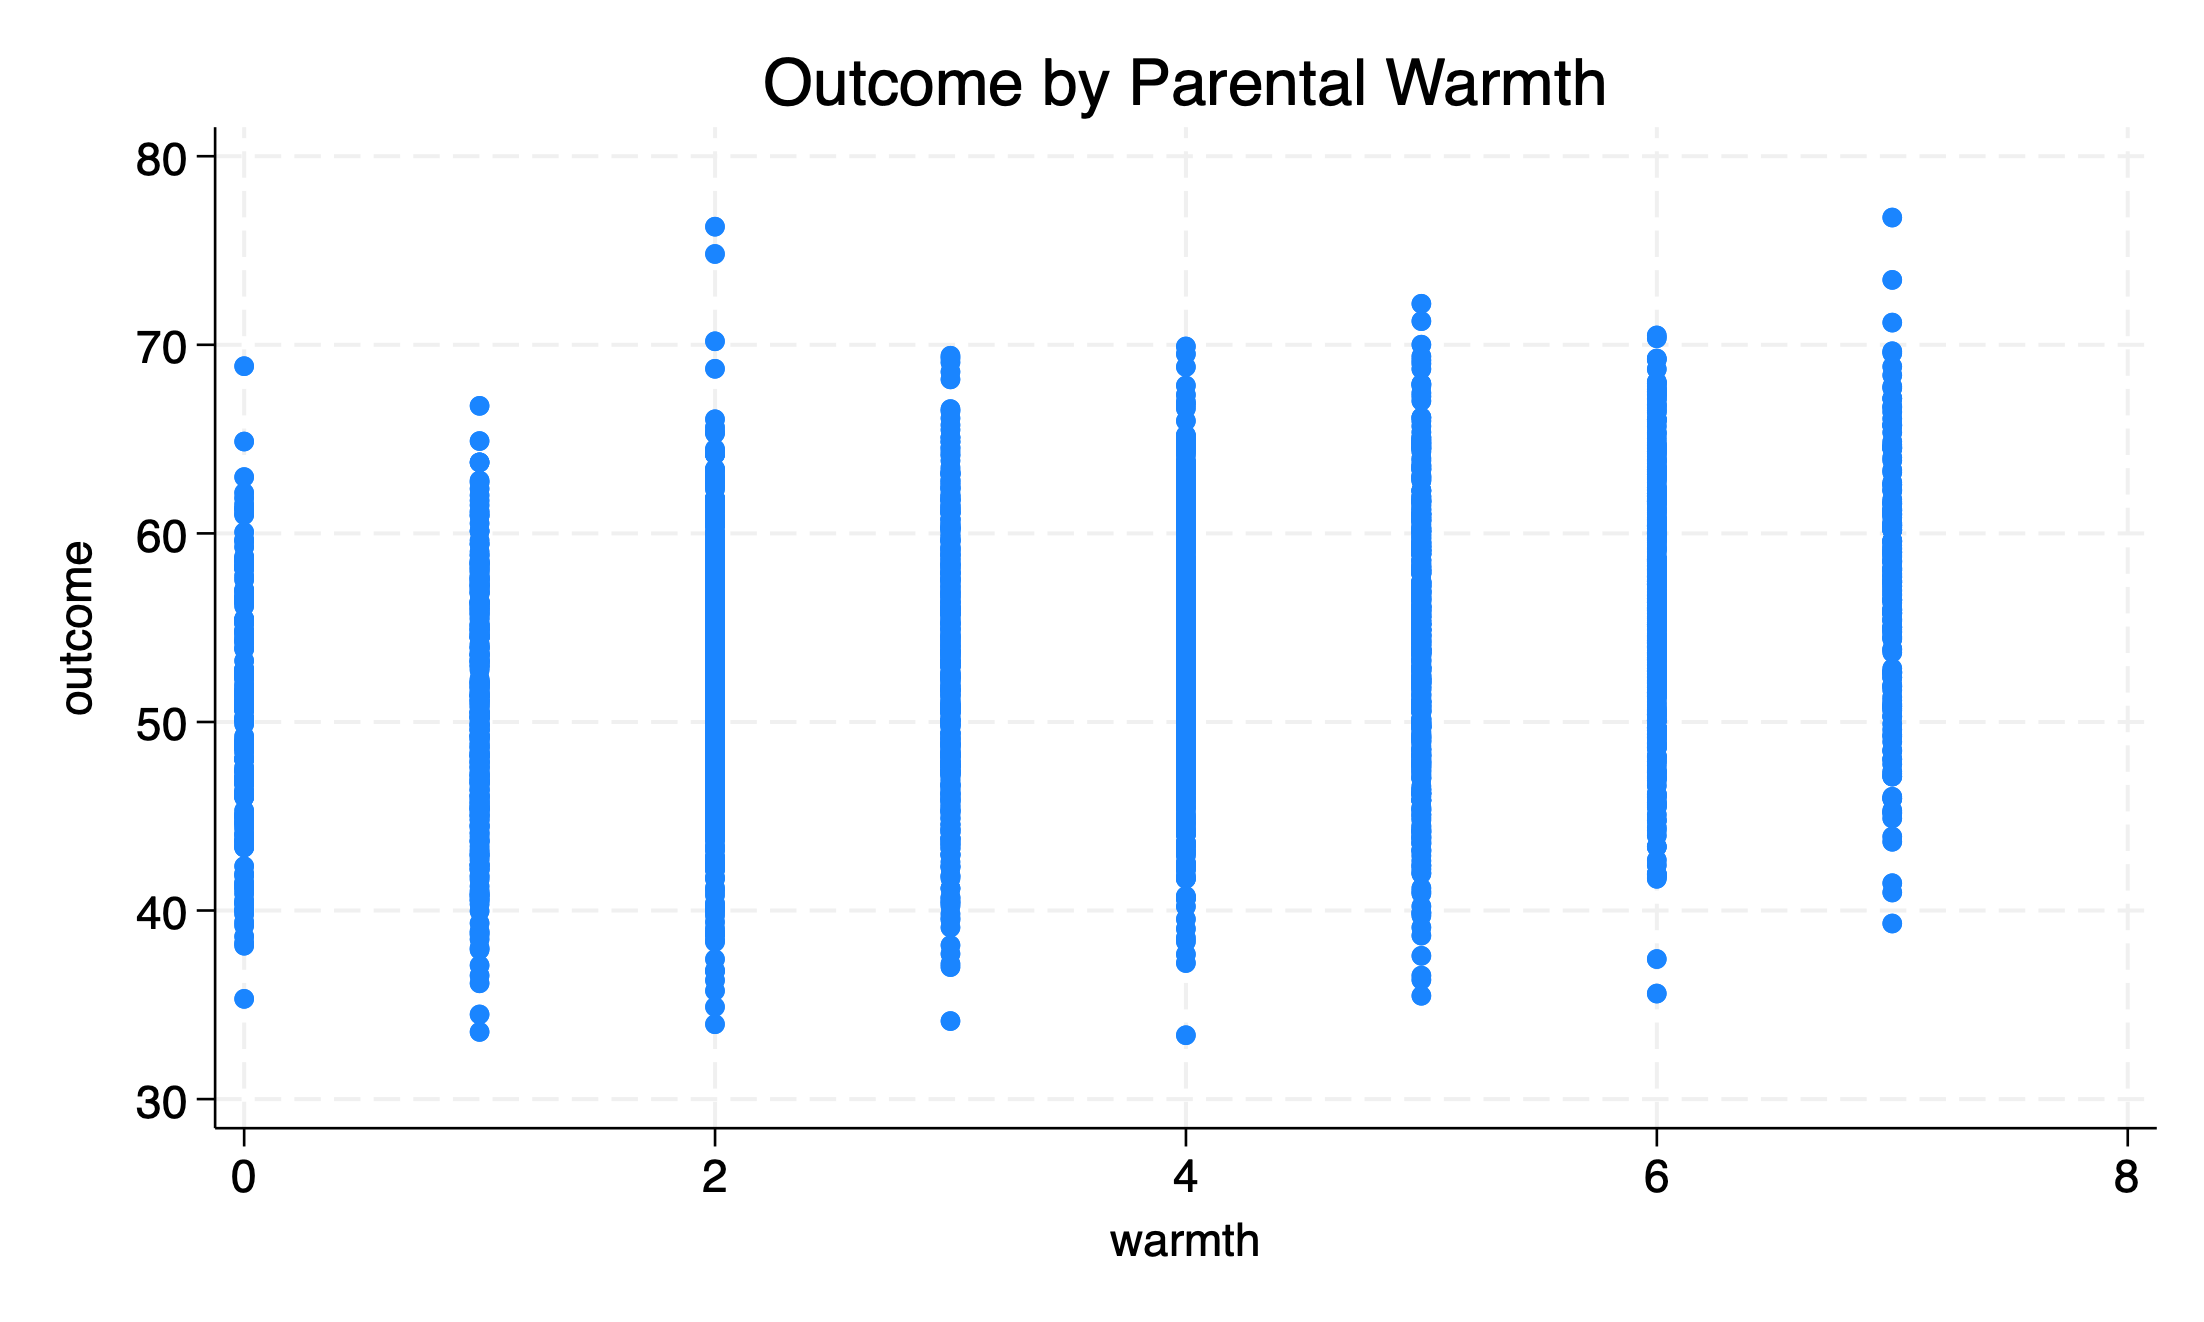
\includegraphics{scatter.png}

}

\caption{Outcome by Parental Warmth}

\end{figure}

\hypertarget{run-the-model}{%
\subsubsection{Run The Model}\label{run-the-model}}

\begin{Shaded}
\begin{Highlighting}[]

\NormalTok{mixed outcome warmth physical\_punishment }\FunctionTok{group}\NormalTok{ HDI || country: warmth}
\end{Highlighting}
\end{Shaded}

\begin{verbatim}
Performing EM optimization ...

Performing gradient-based optimization: 
Iteration 0:  Log likelihood =  -9668.198  
Iteration 1:  Log likelihood = -9667.9551  
Iteration 2:  Log likelihood = -9667.9534  
Iteration 3:  Log likelihood = -9667.9533  
Iteration 4:  Log likelihood = -9667.9532  

Computing standard errors ...

Mixed-effects ML regression                          Number of obs    =  3,000
Group variable: country                              Number of groups =     30
                                                     Obs per group:
                                                                  min =    100
                                                                  avg =  100.0
                                                                  max =    100
                                                     Wald chi2(4)     = 401.26
Log likelihood = -9667.9532                          Prob > chi2      = 0.0000

-------------------------------------------------------------------------------------
            outcome | Coefficient  Std. err.      z    P>|z|     [95% conf. interval]
--------------------+----------------------------------------------------------------
             warmth |   .9616447   .0581825    16.53   0.000     .8476091     1.07568
physical_punishment |  -.8453802   .0798155   -10.59   0.000    -1.001816   -.6889448
              group |   1.084344   .2200539     4.93   0.000     .6530461    1.515642
                HDI |    .010557   .0204522     0.52   0.606    -.0295286    .0506426
              _cons |   49.87963   1.436612    34.72   0.000     47.06392    52.69534
-------------------------------------------------------------------------------------

------------------------------------------------------------------------------
  Random-effects parameters  |   Estimate   Std. err.     [95% conf. interval]
-----------------------------+------------------------------------------------
country: Independent         |
                 var(warmth) |   1.83e-06   .0000173      1.76e-14    190.9774
                  var(_cons) |   3.370262   .9633726      1.924651    5.901676
-----------------------------+------------------------------------------------
               var(Residual) |   36.01906   .9346936      34.23291    37.89842
------------------------------------------------------------------------------
LR test vs. linear model: chi2(2) = 198.01                Prob > chi2 = 0.0000

Note: LR test is conservative and provided only for reference.
\end{verbatim}

\subsection{R}

In R \texttt{lme4}, the general syntax for a multilevel model of the
form described in Equation~\ref{eq-MLMsimple} is:

\texttt{lmer(y\ \textasciitilde{}\ x\ +\ z\ +\ (1\ +\ x\ \textbar{}\textbar{}\ group),\ data\ =\ ...)}

\hypertarget{get-the-data-1}{%
\subsubsection{Get The Data}\label{get-the-data-1}}

\begin{Shaded}
\begin{Highlighting}[]
\FunctionTok{library}\NormalTok{(haven)}

\NormalTok{df }\OtherTok{\textless{}{-}} \FunctionTok{read\_dta}\NormalTok{(}\StringTok{"simulated\_multilevel\_data.dta"}\NormalTok{)}
\end{Highlighting}
\end{Shaded}

\hypertarget{graph-1}{%
\subsubsection{Graph}\label{graph-1}}

\begin{Shaded}
\begin{Highlighting}[]
\FunctionTok{library}\NormalTok{(ggplot2)}

\FunctionTok{ggplot}\NormalTok{(df,}
       \FunctionTok{aes}\NormalTok{(}\AttributeTok{x =}\NormalTok{ warmth,}
           \AttributeTok{y =}\NormalTok{ outcome)) }\SpecialCharTok{+}
  \FunctionTok{geom\_point}\NormalTok{() }\SpecialCharTok{+}
  \FunctionTok{labs}\NormalTok{(}\AttributeTok{title =} \StringTok{"Outcome by Parental Warmth"}\NormalTok{)}
\end{Highlighting}
\end{Shaded}

\begin{figure}[H]

{\centering 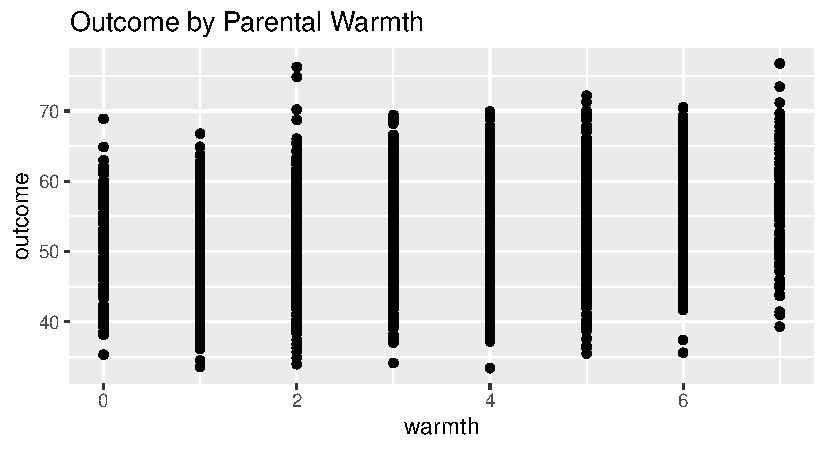
\includegraphics{index_files/figure-pdf/unnamed-chunk-11-1.pdf}

}

\end{figure}

\hypertarget{run-the-model-1}{%
\subsubsection{Run The Model}\label{run-the-model-1}}

\begin{Shaded}
\begin{Highlighting}[]
\NormalTok{fit1 }\OtherTok{\textless{}{-}} \FunctionTok{lmer}\NormalTok{(outcome }\SpecialCharTok{\textasciitilde{}}\NormalTok{ warmth }\SpecialCharTok{+}\NormalTok{ physical\_punishment }\SpecialCharTok{+} 
\NormalTok{               group }\SpecialCharTok{+}\NormalTok{ HDI }\SpecialCharTok{+}
\NormalTok{               (}\DecValTok{1} \SpecialCharTok{+}\NormalTok{ warmth }\SpecialCharTok{||}\NormalTok{ country),}
             \AttributeTok{data =}\NormalTok{ df)}

\FunctionTok{summary}\NormalTok{(fit1)}
\end{Highlighting}
\end{Shaded}

\begin{verbatim}
Linear mixed model fit by REML ['lmerMod']
Formula: outcome ~ warmth + physical_punishment + group + HDI + ((1 |  
    country) + (0 + warmth | country))
   Data: df

REML criterion at convergence: 19350.3

Scaled residuals: 
    Min      1Q  Median      3Q     Max 
-3.4496 -0.6807  0.0016  0.6864  3.1792 

Random effects:
 Groups    Name        Variance  Std.Dev.
 country   (Intercept)  3.611568 1.90041 
 country.1 warmth       0.001876 0.04331 
 Residual              36.049124 6.00409 
Number of obs: 3000, groups:  country, 30

Fixed effects:
                    Estimate Std. Error t value
(Intercept)         49.88754    1.48203  33.662
warmth               0.96155    0.05875  16.367
physical_punishment -0.84556    0.07986 -10.588
group                1.08471    0.22017   4.927
HDI                  0.01044    0.02116   0.493

Correlation of Fixed Effects:
            (Intr) warmth physc_ group 
warmth      -0.126                     
physcl_pnsh -0.135 -0.025              
group       -0.218 -0.010 -0.019       
HDI         -0.925 -0.006  0.008 -0.001
\end{verbatim}

\subsection{Julia}

In Julia \texttt{MixedModels}, the general syntax for a multilevel model
of the form described in Equation~\ref{eq-MLMsimple} is:

\texttt{fit(MixedModel,\ @formula(y\ \textasciitilde{}\ x\ +\ z\ +\ (1\ +\ x\ \textbar{}\ group)),\ data)}

\hypertarget{load-the-needed-packages-and-load-the-data}{%
\subsubsection{Load The Needed Packages And Load The
Data}\label{load-the-needed-packages-and-load-the-data}}

\begin{Shaded}
\begin{Highlighting}[]
\ImportTok{using} \BuiltInTok{Tables}\NormalTok{, }\BuiltInTok{MixedModels}\NormalTok{, }\BuiltInTok{StatFiles}\NormalTok{, }\BuiltInTok{DataFrames}\NormalTok{, }\BuiltInTok{CategoricalArrays}\NormalTok{, }\BuiltInTok{DataFramesMeta}

\NormalTok{df }\OperatorTok{=} \FunctionTok{DataFrame}\NormalTok{(}\FunctionTok{load}\NormalTok{(}\StringTok{"simulated\_multilevel\_data.dta"}\NormalTok{))}
\end{Highlighting}
\end{Shaded}

\hypertarget{graph-2}{%
\subsubsection{Graph}\label{graph-2}}

\begin{Shaded}
\begin{Highlighting}[]
\ImportTok{using} \BuiltInTok{StatsPlots}

\PreprocessorTok{@df}\NormalTok{ df }\FunctionTok{scatter}\NormalTok{(}\OperatorTok{:}\NormalTok{outcome, }\OperatorTok{:}\NormalTok{warmth, }
\NormalTok{               title }\OperatorTok{=} \StringTok{"Outcome by Parental Warmth"}\NormalTok{,}
\NormalTok{               ylabel }\OperatorTok{=} \StringTok{"outcome"}\NormalTok{,}
\NormalTok{               xlabel }\OperatorTok{=} \StringTok{"parental warmth"}\NormalTok{)}
\end{Highlighting}
\end{Shaded}

\begin{figure}[H]

{\centering 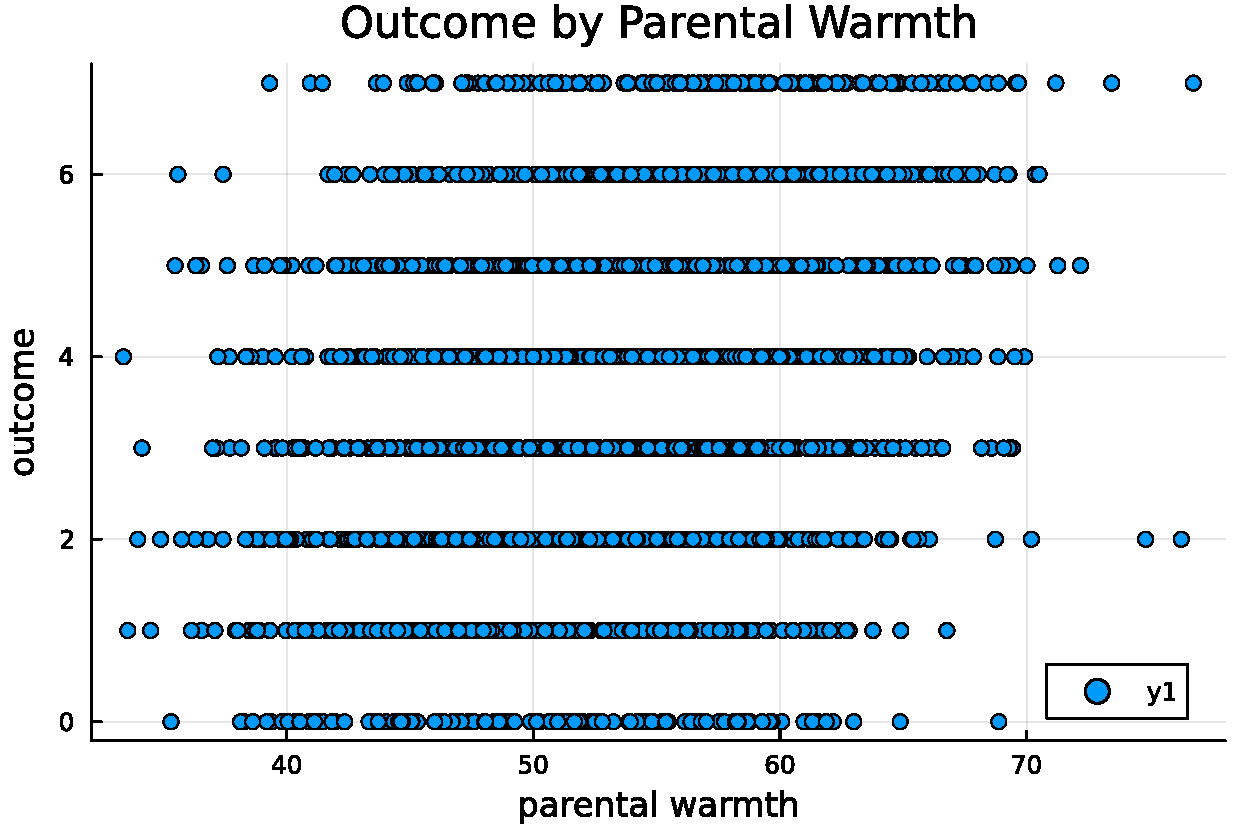
\includegraphics{index_files/figure-pdf/unnamed-chunk-14-J1.pdf}

}

\end{figure}

\hypertarget{change-country-to-categorical}{%
\subsubsection{Change Country To
Categorical}\label{change-country-to-categorical}}

\begin{Shaded}
\begin{Highlighting}[]
\PreprocessorTok{@transform}\NormalTok{!(df, }\OperatorTok{:}\NormalTok{country }\OperatorTok{=} \FunctionTok{categorical}\NormalTok{(}\OperatorTok{:}\NormalTok{country))}
\end{Highlighting}
\end{Shaded}

\hypertarget{run-the-model-2}{%
\subsubsection{Run The Model}\label{run-the-model-2}}

\begin{Shaded}
\begin{Highlighting}[]

\NormalTok{m1 }\OperatorTok{=} \FunctionTok{fit}\NormalTok{(MixedModel, }\PreprocessorTok{@formula}\NormalTok{(outcome }\OperatorTok{\textasciitilde{}}\NormalTok{ warmth }\OperatorTok{+}\NormalTok{ physical\_punishment }\OperatorTok{+} 
\NormalTok{               group }\OperatorTok{+}\NormalTok{ HDI }\OperatorTok{+}
\NormalTok{               (}\FloatTok{1} \OperatorTok{+}\NormalTok{ warmth }\OperatorTok{|}\NormalTok{ country)), df)}
\end{Highlighting}
\end{Shaded}

\begin{verbatim}
Linear mixed model fit by maximum likelihood
 outcome ~ 1 + warmth + physical_punishment + group + HDI + (1 + warmth | country)
   logLik   -2 logLik     AIC       AICc        BIC    
 -9667.9392 19335.8783 19353.8783 19353.9385 19407.9357

Variance components:
            Column    Variance   Std.Dev.   Corr.
country  (Intercept)   3.2369484 1.7991521
         warmth        0.0001080 0.0103903 +1.00
Residual              36.0187144 6.0015593
 Number of obs: 3000; levels of grouping factors: 30

  Fixed-effects parameters:
─────────────────────────────────────────────────────────────
                          Coef.  Std. Error       z  Pr(>|z|)
─────────────────────────────────────────────────────────────
(Intercept)          49.9018      1.43435     34.79    <1e-99
warmth                0.961545    0.0582135   16.52    <1e-60
physical_punishment  -0.845389    0.0798149  -10.59    <1e-25
group                 1.08524     0.220055     4.93    <1e-06
HDI                   0.0101984   0.0204401    0.50    0.6178
─────────────────────────────────────────────────────────────
\end{verbatim}

\bookmarksetup{startatroot}

\hypertarget{cross-classified-models-in-stata-r-and-julia}{%
\chapter{Cross-Classified Models in Stata, R and
Julia}\label{cross-classified-models-in-stata-r-and-julia}}

\hypertarget{introduction-1}{%
\section{Introduction}\label{introduction-1}}

A two level multilevel model imagines that \emph{Level 1} units are
nested in \emph{Level 2} units. A three level multilevel model imagines
that \emph{Level 1} units are nested in \emph{Level 2} units, which are
in turn nested in \emph{Level 3}.

A cross-classified model imagines that the nesting is not hierarchical,
but rather that there are two sets of clusters or nestings in which
individuals may be nested.

In this data, \emph{events} are nested inside \emph{persons} which are
in turn nested in \emph{countries}, since in this data, individuals
never change countries. However, the use of a cross-classified framework
would allow for a situation in which \emph{persons} moved from country
to country, and experienced different \emph{events} in different
\emph{countries}.

Below, I describe the use of \href{https://www.stata.com/}{Stata},
\href{https://www.r-project.org/}{R}, and
\href{https://www.julialang.org/}{Julia} to estimate cross-classified
models. Because this document is built by
\href{https://quarto.org/}{\texttt{Quarto}}, I describe calling these
programs from within a \texttt{Quarto} environment. However, each piece
of software could be used individually and separately.

\hypertarget{the-data-1}{%
\section{The Data}\label{the-data-1}}

\begin{marginfigure}

{\centering 
\includegraphics[width=2.4in,height=\textheight]{bookcover.png}

}

\caption{\label{fig-bookcover}Book Cover For Multilevel Thinking}

\end{marginfigure}

The examples below use the
\texttt{simulated\_multilevel\_longitudinal\_data.dta} file from
\href{https://agrogan1.github.io/multilevel-thinking/simulated-multi-country-data.html}{\emph{Multilevel
Thinking}}. Here is a
\href{https://github.com/agrogan1/multilevel-multilingual/raw/main/simulated_multilevel_longitudinal_data.dta}{direct
link} to download the data.

\hypertarget{tbl-multilingual1}{}
\begin{longtable}[]{@{}
  >{\centering\arraybackslash}p{(\columnwidth - 16\tabcolsep) * \real{0.1190}}
  >{\centering\arraybackslash}p{(\columnwidth - 16\tabcolsep) * \real{0.0714}}
  >{\centering\arraybackslash}p{(\columnwidth - 16\tabcolsep) * \real{0.1071}}
  >{\centering\arraybackslash}p{(\columnwidth - 16\tabcolsep) * \real{0.0714}}
  >{\centering\arraybackslash}p{(\columnwidth - 16\tabcolsep) * \real{0.0952}}
  >{\centering\arraybackslash}p{(\columnwidth - 16\tabcolsep) * \real{0.0476}}
  >{\centering\arraybackslash}p{(\columnwidth - 16\tabcolsep) * \real{0.2619}}
  >{\centering\arraybackslash}p{(\columnwidth - 16\tabcolsep) * \real{0.1071}}
  >{\centering\arraybackslash}p{(\columnwidth - 16\tabcolsep) * \real{0.1190}}@{}}
\caption{\label{tbl-multilingual1}Sample of Simulated Multilevel
Longitudinal Data}\tabularnewline
\toprule\noalign{}
\begin{minipage}[b]{\linewidth}\centering
country
\end{minipage} & \begin{minipage}[b]{\linewidth}\centering
HDI
\end{minipage} & \begin{minipage}[b]{\linewidth}\centering
family
\end{minipage} & \begin{minipage}[b]{\linewidth}\centering
id
\end{minipage} & \begin{minipage}[b]{\linewidth}\centering
group
\end{minipage} & \begin{minipage}[b]{\linewidth}\centering
t
\end{minipage} & \begin{minipage}[b]{\linewidth}\centering
physical\_punishment
\end{minipage} & \begin{minipage}[b]{\linewidth}\centering
warmth
\end{minipage} & \begin{minipage}[b]{\linewidth}\centering
outcome
\end{minipage} \\
\midrule\noalign{}
\endfirsthead
\toprule\noalign{}
\begin{minipage}[b]{\linewidth}\centering
country
\end{minipage} & \begin{minipage}[b]{\linewidth}\centering
HDI
\end{minipage} & \begin{minipage}[b]{\linewidth}\centering
family
\end{minipage} & \begin{minipage}[b]{\linewidth}\centering
id
\end{minipage} & \begin{minipage}[b]{\linewidth}\centering
group
\end{minipage} & \begin{minipage}[b]{\linewidth}\centering
t
\end{minipage} & \begin{minipage}[b]{\linewidth}\centering
physical\_punishment
\end{minipage} & \begin{minipage}[b]{\linewidth}\centering
warmth
\end{minipage} & \begin{minipage}[b]{\linewidth}\centering
outcome
\end{minipage} \\
\midrule\noalign{}
\endhead
\bottomrule\noalign{}
\endlastfoot
1 & 69 & 1 & 1.1 & 2 & 1 & 2 & 3 & 59.18 \\
1 & 69 & 1 & 1.1 & 2 & 2 & 2 & 2 & 58.29 \\
1 & 69 & 1 & 1.1 & 2 & 3 & 3 & 3 & 60.58 \\
1 & 69 & 2 & 1.2 & 2 & 1 & 4 & 0 & 61.54 \\
1 & 69 & 2 & 1.2 & 2 & 2 & 4 & 0 & 55.96 \\
1 & 69 & 2 & 1.2 & 2 & 3 & 4 & 2 & 56.19 \\
\end{longtable}

\hypertarget{the-equation-1}{%
\section{The Equation}\label{the-equation-1}}

\begin{equation}\protect\hypertarget{eq-crossclassifiedsubstantive}{}{\begin{gather} \text{outcome}_{ijt}= \beta_0 + \beta_1 t_{ijt} + \beta_2 \text{warmth}_{ijt} + \beta_3 \text{physical punishment}_{ijt} + \\ \beta_4 \text{group}_{ijt} + \beta_5 \text{HDI}_{ijt} + \\ u_{0j} + v_{0i} + e_{ijt} \end{gather}}\label{eq-crossclassifiedsubstantive}\end{equation}

\hypertarget{setup-1}{%
\section{Setup}\label{setup-1}}

\subsection{Stata}

I need to use the library \texttt{Statamarkdown} to call Stata, or I
could run Stata on its own

\begin{Shaded}
\begin{Highlighting}[]
\FunctionTok{library}\NormalTok{(Statamarkdown)}
\end{Highlighting}
\end{Shaded}

\subsection{R}

In R, I use the library \texttt{lme4} to run multilevel models.

\begin{Shaded}
\begin{Highlighting}[]
\FunctionTok{library}\NormalTok{(lme4)}
\end{Highlighting}
\end{Shaded}

\subsection{Julia}

I need to call Julia from R.

\begin{Shaded}
\begin{Highlighting}[]
\FunctionTok{library}\NormalTok{(JuliaCall)}

\FunctionTok{julia\_setup}\NormalTok{(}\AttributeTok{JULIA\_HOME =} \StringTok{"/Applications/Julia{-}1.8.app/Contents/Resources/julia/bin"}\NormalTok{)}
\end{Highlighting}
\end{Shaded}

\hypertarget{get-data-run-models-1}{%
\section{Get Data \& Run Models}\label{get-data-run-models-1}}

To explain statistical syntax for each software, I consider the more
general case of a cross-classified model with dependent variable
\texttt{y}, independent variables \texttt{x} and \texttt{z}, clustering
variables \texttt{country} and \texttt{id}.

\begin{equation}\protect\hypertarget{eq-crossclassfiedsimple}{}{y = \beta_0 + \beta_1 x_{ijt} + \beta_2 z_{ijt} + u_{0j} + v_{0i} + e_{ijt}}\label{eq-crossclassfiedsimple}\end{equation}

\subsection{Stata}

In Stata \texttt{mixed}, the syntax for a multilevel model of the form
described in Equation~\ref{eq-crossclassfiedsimple} is:

\texttt{mixed\ y\ x\ \textbar{}\textbar{}\ \_all:\ R.group1\ \textbar{}\textbar{}\ group2:}

\hypertarget{get-the-data-2}{%
\subsubsection{Get The Data}\label{get-the-data-2}}

\begin{tcolorbox}[enhanced jigsaw, arc=.35mm, coltitle=black, bottomtitle=1mm, colbacktitle=quarto-callout-tip-color!10!white, opacityback=0, colback=white, colframe=quarto-callout-tip-color-frame, opacitybacktitle=0.6, breakable, title=\textcolor{quarto-callout-tip-color}{\faLightbulb}\hspace{0.5em}{Tip For Running Stata From Quarto}, leftrule=.75mm, toptitle=1mm, bottomrule=.15mm, rightrule=.15mm, titlerule=0mm, toprule=.15mm, left=2mm]

Because I am running Stata from inside a Quarto document, and running
Stata in multiple chunks, I need to use the \texttt{collectcode=TRUE}
option in the first Stata chunk. i.e.~my Quarto chunk needs to begin
with ```\texttt{\{stata,\ collectcode=TRUE\}}

See Doug Hemken's excellent documentation on \texttt{Statamarkdown}
\href{https://www.ssc.wisc.edu/~hemken/Stataworkshops/Statamarkdown/linking-code-blocks.html\#linking-code-blocks-1}{here}.

\end{tcolorbox}

\begin{Shaded}
\begin{Highlighting}[]

\KeywordTok{use}\NormalTok{ simulated\_multilevel\_longitudinal\_data.dta}
\end{Highlighting}
\end{Shaded}

\hypertarget{run-the-model-3}{%
\subsubsection{Run The Model}\label{run-the-model-3}}

\begin{Shaded}
\begin{Highlighting}[]

\NormalTok{mixed outcome t warmth physical\_punishment }\FunctionTok{group}\NormalTok{ HDI || }\DataTypeTok{\_all}\NormalTok{: R.country || id:}
\end{Highlighting}
\end{Shaded}

\begin{verbatim}
Performing EM optimization ...

Performing gradient-based optimization: 
Iteration 0:  Log likelihood = -28534.027  
Iteration 1:  Log likelihood = -28533.997  
Iteration 2:  Log likelihood = -28533.997  

Computing standard errors ...

Mixed-effects ML regression                            Number of obs =   9,000

        Grouping information
        -------------------------------------------------------------
                        |     No. of       Observations per group
         Group variable |     groups    Minimum    Average    Maximum
        ----------------+--------------------------------------------
                   _all |          1      9,000    9,000.0      9,000
                     id |      3,000          3        3.0          3
        -------------------------------------------------------------

                                                       Wald chi2(5)  = 1206.21
Log likelihood = -28533.997                            Prob > chi2   =  0.0000

-------------------------------------------------------------------------------------
            outcome | Coefficient  Std. err.      z    P>|z|     [95% conf. interval]
--------------------+----------------------------------------------------------------
                  t |   .9879647   .0658315    15.01   0.000     .8589373    1.116992
             warmth |   .9462548   .0381869    24.78   0.000     .8714098      1.0211
physical_punishment |  -.9267739   .0499549   -18.55   0.000    -1.024684    -.828864
              group |    .985819   .1534866     6.42   0.000     .6849908    1.286647
                HDI |   .0075436   .0207106     0.36   0.716    -.0330485    .0481356
              _cons |   49.49447   1.424253    34.75   0.000     46.70299    52.28596
-------------------------------------------------------------------------------------

------------------------------------------------------------------------------
  Random-effects parameters  |   Estimate   Std. err.     [95% conf. interval]
-----------------------------+------------------------------------------------
_all: Identity               |
              var(R.country) |   3.650496   .9878413      2.147893    6.204274
-----------------------------+------------------------------------------------
id: Identity                 |
                  var(_cons) |   8.852634   .4815279      7.957424    9.848556
-----------------------------+------------------------------------------------
               var(Residual) |   26.00093   .4747632      25.08686     26.9483
------------------------------------------------------------------------------
LR test vs. linear model: chi2(2) = 1328.22               Prob > chi2 = 0.0000

Note: LR test is conservative and provided only for reference.
\end{verbatim}

\subsection{R}

In R \texttt{lme4}, the general syntax for a multilevel model of the
form described in Equation~\ref{eq-crossclassfiedsimple} is:

\texttt{lmer(y\ \textasciitilde{}\ x\ +\ z\ +\ (1\ \textbar{}\ group1)\ +\ (1\ \textbar{}\ group2),\ data\ =\ ...)}

\hypertarget{get-the-data-3}{%
\subsubsection{Get The Data}\label{get-the-data-3}}

\begin{Shaded}
\begin{Highlighting}[]
\FunctionTok{library}\NormalTok{(haven)}

\NormalTok{df }\OtherTok{\textless{}{-}} \FunctionTok{read\_dta}\NormalTok{(}\StringTok{"simulated\_multilevel\_longitudinal\_data.dta"}\NormalTok{)}
\end{Highlighting}
\end{Shaded}

\hypertarget{run-the-model-4}{%
\subsubsection{Run The Model}\label{run-the-model-4}}

\begin{Shaded}
\begin{Highlighting}[]
\NormalTok{fit1 }\OtherTok{\textless{}{-}} \FunctionTok{lmer}\NormalTok{(outcome }\SpecialCharTok{\textasciitilde{}}\NormalTok{ t }\SpecialCharTok{+}\NormalTok{ warmth }\SpecialCharTok{+}\NormalTok{ physical\_punishment }\SpecialCharTok{+} 
\NormalTok{               group }\SpecialCharTok{+}\NormalTok{ HDI }\SpecialCharTok{+}
\NormalTok{               (}\DecValTok{1} \SpecialCharTok{|}\NormalTok{ id) }\SpecialCharTok{+}
\NormalTok{               (}\DecValTok{1} \SpecialCharTok{|}\NormalTok{ country),}
             \AttributeTok{data =}\NormalTok{ df)}

\FunctionTok{summary}\NormalTok{(fit1)}
\end{Highlighting}
\end{Shaded}

\begin{verbatim}
Linear mixed model fit by REML ['lmerMod']
Formula: outcome ~ t + warmth + physical_punishment + group + HDI + (1 |  
    id) + (1 | country)
   Data: df

REML criterion at convergence: 57088.4

Scaled residuals: 
    Min      1Q  Median      3Q     Max 
-3.4471 -0.6226  0.0081  0.6153  3.1993 

Random effects:
 Groups   Name        Variance Std.Dev.
 id       (Intercept)  8.864   2.977   
 country  (Intercept)  3.924   1.981   
 Residual             26.008   5.100   
Number of obs: 9000, groups:  id, 3000; country, 30

Fixed effects:
                     Estimate Std. Error t value
(Intercept)         49.494782   1.471780  33.629
t                    0.987964   0.065840  15.005
warmth               0.946259   0.038200  24.771
physical_punishment -0.926880   0.049970 -18.549
group                0.985786   0.153550   6.420
HDI                  0.007543   0.021437   0.352

Correlation of Fixed Effects:
            (Intr) t      warmth physc_ group 
t           -0.090                            
warmth      -0.085  0.008                     
physcl_pnsh -0.085  0.003 -0.019              
group       -0.154  0.000 -0.013 -0.008       
HDI         -0.943  0.000 -0.003  0.003  0.000
\end{verbatim}

\subsection{Julia}

In Julia \texttt{MixedModels}, the general syntax for a multilevel model
of the form described in Equation~\ref{eq-crossclassfiedsimple} is:

\texttt{fit(MixedModel,\ @formula(y\ \textasciitilde{}\ x\ +\ z\ +\ (1\ \textbar{}\ group1)\ +\ (1\ \textbar{}\ group2)),\ data)}

\hypertarget{load-the-needed-packages-and-load-the-data-1}{%
\subsubsection{Load The Needed Packages And Load The
Data}\label{load-the-needed-packages-and-load-the-data-1}}

\begin{Shaded}
\begin{Highlighting}[]
\ImportTok{using} \BuiltInTok{Tables}\NormalTok{, }\BuiltInTok{MixedModels}\NormalTok{, }\BuiltInTok{StatFiles}\NormalTok{, }\BuiltInTok{DataFrames}\NormalTok{, }\BuiltInTok{CategoricalArrays}\NormalTok{, }\BuiltInTok{DataFramesMeta}

\NormalTok{df }\OperatorTok{=} \FunctionTok{DataFrame}\NormalTok{(}\FunctionTok{load}\NormalTok{(}\StringTok{"simulated\_multilevel\_longitudinal\_data.dta"}\NormalTok{))}
\end{Highlighting}
\end{Shaded}

\hypertarget{change-country-to-categorical-1}{%
\subsubsection{Change Country To
Categorical}\label{change-country-to-categorical-1}}

\begin{Shaded}
\begin{Highlighting}[]
\PreprocessorTok{@transform}\NormalTok{!(df, }\OperatorTok{:}\NormalTok{country }\OperatorTok{=} \FunctionTok{categorical}\NormalTok{(}\OperatorTok{:}\NormalTok{country))}
\end{Highlighting}
\end{Shaded}

\hypertarget{run-the-model-5}{%
\subsubsection{Run The Model}\label{run-the-model-5}}

\begin{Shaded}
\begin{Highlighting}[]

\NormalTok{m1 }\OperatorTok{=} \FunctionTok{fit}\NormalTok{(MixedModel, }\PreprocessorTok{@formula}\NormalTok{(outcome }\OperatorTok{\textasciitilde{}}\NormalTok{ t }\OperatorTok{+}\NormalTok{ warmth }\OperatorTok{+}\NormalTok{ physical\_punishment }\OperatorTok{+} 
\NormalTok{                                group }\OperatorTok{+}\NormalTok{ HDI }\OperatorTok{+}
\NormalTok{                                (}\FloatTok{1} \OperatorTok{|}\NormalTok{ id) }\OperatorTok{+}
\NormalTok{                                (}\FloatTok{1} \OperatorTok{|}\NormalTok{ country)), df)}
\end{Highlighting}
\end{Shaded}

\begin{verbatim}
Linear mixed model fit by maximum likelihood
 outcome ~ 1 + t + warmth + physical_punishment + group + HDI + (1 | id) + (1 | country)
    logLik   -2 logLik      AIC         AICc        BIC     
 -28533.9968  57067.9935  57085.9935  57086.0136  57149.9384

Variance components:
            Column   Variance Std.Dev.
id       (Intercept)   8.85264 2.97534
country  (Intercept)   3.65030 1.91058
Residual              26.00093 5.09911
 Number of obs: 9000; levels of grouping factors: 3000, 30

  Fixed-effects parameters:
──────────────────────────────────────────────────────────────
                           Coef.  Std. Error       z  Pr(>|z|)
──────────────────────────────────────────────────────────────
(Intercept)          49.4945       1.42422     34.75    <1e-99
t                     0.987965     0.0658315   15.01    <1e-50
warmth                0.946255     0.0381869   24.78    <1e-99
physical_punishment  -0.926774     0.0499549  -18.55    <1e-76
group                 0.985819     0.153487     6.42    <1e-09
HDI                   0.00754357   0.0207101    0.36    0.7157
──────────────────────────────────────────────────────────────
\end{verbatim}



\end{document}
